\subsection{CAD Design for Central Motor Sprocket}
\begin{figure}[h!]
	\centering
   	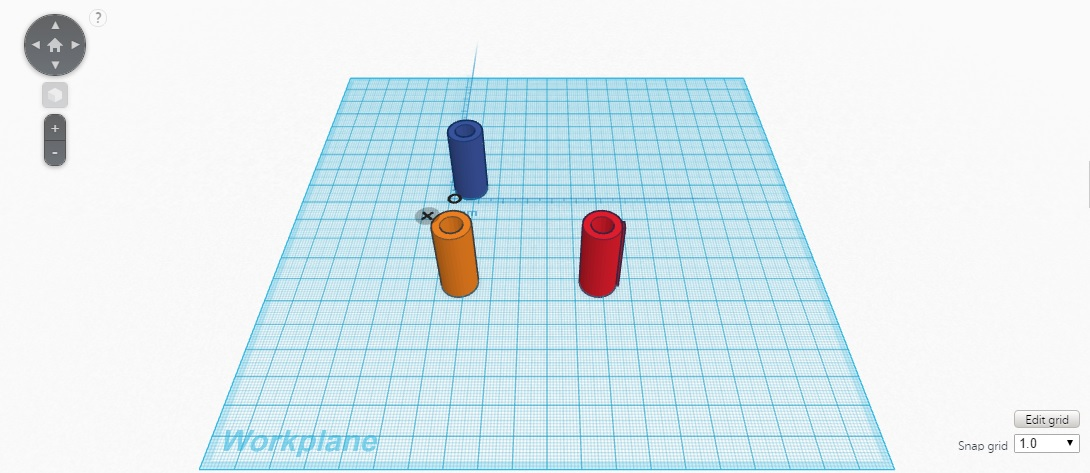
\includegraphics[width=0.60\textwidth]{images/CADimg}
\end{figure}

\subsection{Joystick Input Test Code}
\begin{verbatim}
//A0(15) = green, A1(16) = yellow, A2(17) = orange, A3(18) = red
#define downPin 15
#define upPin 16
#define rightPin 17
#define leftPin 18
int X = 0;
int Y = 0;
int PrevX = X;
int PrevY = Y;
 
void setup() {
  Serial.begin(9600);
  
  //Joystick setup
  pinMode(downPin, INPUT);
  digitalWrite(downPin, HIGH);
  pinMode(upPin, INPUT);
  digitalWrite(upPin, HIGH);
  pinMode(rightPin, INPUT);
  digitalWrite(rightPin, HIGH);
  pinMode(leftPin, INPUT);
  digitalWrite(leftPin, HIGH);
}

void loop() {
  joystick( &X, &Y );
  if (X != 0 && (X != PrevX || Y != PrevY)){
    result(X,Y);
  }
  else if (Y != 0 && (X != PrevX || Y != PrevY)) {
    result(X,Y);
  }
  delay(300);
}

// [-1, 0, 1] map to [left/down, none, right/top]
void joystick(int* X, int* Y){

  //HIGH = non-trigger
  if( !digitalRead( leftPin ) ){
    *X = -1;
  }else if( !digitalRead( rightPin ) ){
    *X = 1;
  }else{
    *X = 0;
  }

  if( !digitalRead( upPin ) ){
    *Y = 1;
  }else if( !digitalRead( downPin ) ){
    *Y = -1;
  }else{
    *Y = 0;
  }

}

void result(int X, int Y ) {
    if (X == 1){
      Serial.print("Right\t");
    }
    else if (X == -1) {
      Serial.print("Left\t");   
    }
    PrevX = X;
    if (Y == 1){
      Serial.print("Up\n");
    }
    else if (Y == -1) {
      Serial.print("Down\n");
    }
    else{
      Serial.print("\n");
    }          
    PrevY = Y;
}
\end{verbatim}

\subsection{Motor Driver Test Code}
\begin{verbatim}
/* LED Blink, Teensyduino Tutorial #1
   http://www.pjrc.com/teensy/tutorial.html
 
   This example code is in the public domain.
*/

// Teensy 2.0 has the LED on pin 11
// Teensy++ 2.0 has the LED on pin 6
// Teensy 3.x / Teensy LC have the LED on pin 13

//A0(15) = green, A1(16) = yellow, A2(17) = orange, A3(18) = red
const int LED_PIN = 13;
const int PWM_PIN = 14;
const int DIR_PIN = 10;
const int HB_PWM = 3;
const int HB_INA = 4;
const int HB_INB = 5;
const int DOWN_PIN = 15;
const int UP_PIN = 16;
const int RIGHT_PIN = 17;
const int LEFT_PIN = 18;
int X = 0;
int Y = 0;
int PrevX = X;
int PrevY = Y;

// the setup() method runs once, when the sketch starts
void setup() {
  // initialize the digital pin as an output.  
   Serial.begin(9600);
  
  pinMode(LED_PIN, OUTPUT);
  pinMode(PWM_PIN, OUTPUT);
  pinMode(DIR_PIN, OUTPUT);
  pinMode(HB_PWM, OUTPUT);
  pinMode(HB_INA, OUTPUT);
  pinMode(HB_INB, OUTPUT);
  pinMode(DOWN_PIN, INPUT);
  pinMode(UP_PIN, INPUT);
  pinMode(RIGHT_PIN, INPUT);
  pinMode(LEFT_PIN, INPUT);
  
  for(int i = 0; i < 25; i++)
  {
    digitalWrite(LED_PIN, HIGH);
    delay(50);
    digitalWrite(LED_PIN, LOW);
    delay(50);
  }
  
  digitalWrite(PWM_PIN, LOW);
  digitalWrite(DOWN_PIN, HIGH); 
  digitalWrite(UP_PIN, HIGH); 
  digitalWrite(RIGHT_PIN, HIGH); 
  digitalWrite(LEFT_PIN, HIGH); 
}

// the loop() methor runs over and over again,
// as long as the board has power
// pwm low = off
// 0 forward
void loop() {  
  joystick( &X, &Y );
  if (X != 0 && (X != PrevX || Y != PrevY)){
    result(X,Y);
  }
  else if (Y != 0 && (X != PrevX || Y != PrevY)) {
    result(X,Y);
  }
  delay(300);
}

void joystick(int* X, int* Y){
  //HIGH = non-trigger
  if( !digitalRead( LEFT_PIN ) ){
    *X = -1;
    turnLeft();
  }else if( !digitalRead( RIGHT_PIN ) ){
    *X = 1;
    turnRight();
  }else{
    *X = 0;
  }

  if( !digitalRead( UP_PIN ) ){
    *Y = 1;
    moveForward();
  }else if( !digitalRead( DOWN_PIN ) ){
    *Y = -1;
    moveBackward();
  }else{
    *Y = 0;
  }
}

void result(int X, int Y ) {
    if (X == 1){
      Serial.print("Right\t");
    }
    else if (X == -1) {
      Serial.print("Left\t");   
    }
    PrevX = X;
    if (Y == 1){
      Serial.print("Up\n");
    }
    else if (Y == -1) {
      Serial.print("Down\n");
    }
    else{
      Serial.print("\n");
    }          
    PrevY = Y;
}

void turnLeft() {
  digitalWrite(HB_PWM, HIGH);    
  digitalWrite(HB_INA, LOW); 
  digitalWrite(HB_INB, HIGH); 
  delay(1350); 
  digitalWrite(HB_PWM, LOW); 
}

void turnRight() {
  digitalWrite(HB_PWM, HIGH); 
  digitalWrite(HB_INB, LOW); 
  digitalWrite(HB_INA, HIGH);
  delay(1350); 
  digitalWrite(HB_PWM, LOW);
}

void moveForward() {
  digitalWrite(PWM_PIN, HIGH);
  digitalWrite(DIR_PIN, HIGH);
  delay(1000);
  digitalWrite(PWM_PIN, LOW);
}

void moveBackward() {
  digitalWrite(PWM_PIN, HIGH);
  digitalWrite(DIR_PIN, LOW);
  delay(1000);
  digitalWrite(PWM_PIN, LOW);
}
\end{verbatim}

\subsection{Final Demo Code}
\begin{verbatim}
const int LED_PIN = 13;
const int PWM_PIN = 10;
const int DIR_PIN = 14;
const int HB_PWM = 3;
const int HB_INA = 4;
const int HB_INB = 5;
const int DOWN_PIN = 15;
const int UP_PIN = 16;
const int RIGHT_PIN = 17;
const int LEFT_PIN = 18;

int X = 0;
int Y = 0;
int PrevX = X;
int PrevY = Y;

void setup() {
  Serial.begin(9600);
  
  pinMode(LED_PIN, OUTPUT);
  pinMode(PWM_PIN, OUTPUT);
  pinMode(DIR_PIN, OUTPUT);
  pinMode(HB_PWM, OUTPUT);
  pinMode(HB_INA, OUTPUT);
  pinMode(HB_INB, OUTPUT);
  pinMode(DOWN_PIN, INPUT);
  pinMode(UP_PIN, INPUT);
  pinMode(RIGHT_PIN, INPUT);
  pinMode(LEFT_PIN, INPUT);
  
  for(int i = 0; i < 25; i++)
  {
    digitalWrite(LED_PIN, HIGH);
    delay(50);
    digitalWrite(LED_PIN, LOW);
    delay(50);
  }

  analogWrite(HB_PWM, LOW);
  digitalWrite(PWM_PIN, LOW);
  digitalWrite(DOWN_PIN, HIGH); 
  digitalWrite(UP_PIN, HIGH); 
  digitalWrite(RIGHT_PIN, HIGH); 
  digitalWrite(LEFT_PIN, HIGH); 
}

void loop() {
  joystick( &X, &Y );
  if (X == 0  && Y == 0){
    stopMoving();
  }
  if (X != 0 && Y != 0){    
    result(X,Y);
  }
 /* stopMoving();
  delay(3000);
  moveForward();
  delay(2000);
  stopMoving();
  delay(3000);
  moveBackward();
  delay(2000);*/
}

void joystick(int* X, int* Y){
  if( !digitalRead( UP_PIN ) ){
      *Y = 1;
      moveForward();
  } else if( !digitalRead( DOWN_PIN ) ){
      *Y = -1;
      moveBackward();
  } else{
      *Y = 0;
  }

  if( !digitalRead( LEFT_PIN ) ){
    *X = -1;
    if (*Y == -1){
      turnLeft();
    } else {
        turnRight();
    }
  } else if( !digitalRead( RIGHT_PIN ) ){
    *X = 1;
    if (*Y == -1){
      turnRight();
    }
    else {
      turnLeft();
    }
  } else{
    *X = 0;
  }
}

void result(int X, int Y ) {
    Serial.print( "X = ");
    Serial.print(X);
    Serial.print(" Y = ");
    Serial.print(Y);
    Serial.print('\n');
    
    PrevX = X;
    PrevY = Y;
}

void turnLeft(){
  digitalWrite(HB_PWM, HIGH);
  digitalWrite(HB_INA, LOW);
  digitalWrite(HB_INB, HIGH);
}

void turnRight(){
  digitalWrite(HB_PWM, HIGH);
  digitalWrite(HB_INB, LOW);
  digitalWrite(HB_INA, HIGH);
}

void moveForward(){
  analogWrite(PWM_PIN, 80);
  digitalWrite(DIR_PIN, HIGH);
}

void moveBackward(){
  analogWrite(PWM_PIN, 80);
  digitalWrite(DIR_PIN, LOW);
}

void stopMoving(){
 analogWrite(PWM_PIN, LOW);
 digitalWrite(HB_PWM, LOW); 
 digitalWrite(HB_INA, LOW); 
 digitalWrite(HB_INB, LOW); 
}
\end{verbatim}
